\chapter{必要工具}

\begin{quote}
    我所爱的,你何其美好。何其可悦,使人欢畅喜乐。你的身量好像棕树。你的两乳如同其上的果子,累累下垂。

    \hfill《圣经·雅歌》7:7
\end{quote}

在本章,我们会介绍创造比第4章中介绍的指令和环境更复杂的指令和环境所需准备的工具。此外,借着本章的介绍,我们旨在说明,此处提到的第4章需要正确消化,才能继续这一部分的阅读。本章也会介绍一些关于字体的机制,以及挖掘\LaTeX 资源的方法。

\section{赫尔克里·波洛}

\subsection{在文件中挖掘信息}

首先,为了让使用\LaTeX 写成的文档带有一些个人特色,需要知道组成你使用的\TeX 或\LaTeX 的发行版的文件的组织方法。鄙人使用了UNIX平台的发行版\TeX Live(\wz{http://www.tug.org/texlive})。在这个发行版中,我们可以在第一时间在以下目录中查阅各种包的文档:

\begin{dmd}
/usr/share/texmf-texlive/doc/latex/
\end{dmd}

这个目录中包含其他子目录,通常每个子目录对应一个包,其中就以DVI或PostScript文件的形式提供了文档。在一些情况下,需要去检查这些包的源代码。在发行版te\TeX 中,这些源代码位于:

\begin{dmd}
/usr/share/texmf-texlive/tex/latex
\end{dmd}

在同样的位置,我们通常可以为每个包找到一个目录,包含文本形式且带有扩展名\dm{sty}的源代码,在必要时也会包含相关文件。最后,为了独立于我们可以包含的包而了解\LaTeX 的默认行为,可以借助以下位置的\LaTeX 源代码:

\begin{dmd}
/usr/share/texmf-texlive/tex/latex/base/latex.ltx
\end{dmd}

对于文档类型\dm{book},还可以借助以下位置的文档类型源代码:

\begin{dmd}
/usr/share/texmf-texlive/tex/latex/base/book.cls
\end{dmd}

\subsection{检查宏}

查找指令定义的一个非常便捷的方法是在交互式会话中求助于\LaTeX 。可以直接在操作系统的命令行终端中执行以下指令:

\dmh{latex}

我的系统是这样冷冰冰地回答的:

\begin{dmd}
\begin{verbatim}
This is e-TeXk, Version 3.14159-2.1 (Web2C 7.4.5)
%&-line parsing enabled.
**
\end{verbatim}
\end{dmd}

在“赤裸裸的\TeX ”呼喊出这个冷峻的提示(\dm{**})的邀请下,我勇敢地回复了\verb|&latex|来要求加载\LaTeX 格式。没有丝毫延迟,就得到了答复:

\begin{dmd}
\begin{verbatim}
**&latex
entering extended mode
LaTeX2e <2001/06/01>
Babel <v3.7h> and hyphenation patterns for american,
french loaded.
*
\end{verbatim}
\end{dmd}

注意,提示中少了一个星号。从现在开始,我们就可以交互式地编写\LaTeX 文档了。从绝对意义商来说,这样做的乐趣不大,但从获取指令的定义和语法上来说,却很有帮助。因此,举例来说,我们可以写下这样的指令:

\begin{dmd}
\verb|*\show|\codereplace{指令}
\end{dmd}

这样可以获取\codereplace{指令}的定义。例如:

\begin{dmd}
\begin{verbatim}
*\show\mbox
> \mbox=\long macro:
\end{verbatim}
\verb|#1->\leavevmode \hbox {#1}.| \quad $\leftarrow$\textsf{此处为定义}\\
\verb+<*> \show\mbox+
\end{dmd}

其中向我们提供了指令\verb|\mbox|的定义。可以注意到,该指令被调用时,将这种调用转化为对\verb|\leavevmode|和\verb|\hbox|的调用。在好奇心的驱使下,我们继续查看指令的定义:

\begin{dmd}
\verb|*\show\hbox|\\
\verb|> \hbox=\hbox.| \quad $\leftarrow$\textsf{这是一个原语}\\
\verb|<*> \show\hbox|
\end{dmd}

可以观察到,\verb|\hbox|不是由其他指令定义而成的。在\TeX 中,这种指令称为原语(primitive)。我们的探索可以继续:

\begin{dmd}
\verb|*\show\leavevmode|\\
\verb|> \leavevmode=macro:|\\
\verb|->\unhbox \voidb@x .|\quad $\leftarrow$\backslash leavevmode\textsf{的定义}\\
\verb|<*> \show\leavevmode|
\end{dmd}

以此类推……

\section{底层工具}

\subsection{百分号图个什么?}

你可能已经注意到,有时\LaTeX 源代码中的行末带有百分号\dm{\%}。基于代码换行时文本间会自动添加空格这样的情况,百分号就有理由出现了。请看如下指令:

\begin{dmd}
\verb|\newcommand{\beurk}{bidule}|
\end{dmd}

为了增强可读性,这条指令可以拆分为多行代码:

\begin{codelist}[9.1]{
\newcommand{\beurk}{
    bidule
}
==(\beurk)==
}\begin{verbatim}
\newcommand{\beurk}{
    bidule
}
==(\beurk)==
\end{verbatim}
\end{codelist}

可以观察到,“bidule”一词的两侧出现了我们不想要的空格。为了避免这种现象,可以使用如下方式改写:


\begin{codelist}[9.2]{
\newcommand{\beurk}{%
    bidule%
}
==(\beurk)==
}\begin{verbatim}
\newcommand{\beurk}{%
    bidule%
}
==(\beurk)==
\end{verbatim}
\end{codelist}

在另一些场景下,空格会为行文带来有害的干预。定义以下环境:

\begin{dmd}
\begin{verbatim}
\newenvironment{hyperimportant}{% 
    \bfseries\itshape}{% 
    \upshape\mdseries}
\end{verbatim}
\end{dmd}

\newenvironment{hyperimportant}{% 
    \bfseries\itshape}{% 
    \upshape\mdseries}

\begin{codelist}[9.3]{
    Il est impératif
\begin{hyperimportant}
  de multiplier les sauvegardes
\end{hyperimportant}
de vos documents personnels
}\begin{verbatim}
Il est impératif
\begin{hyperimportant}
    de multiplier les sauvegardes
\end{hyperimportant}
de vos documents personnels
\end{verbatim}
\end{codelist}

如果仔细观察生成的文本,可以注意到,在粗斜体部分文本“{\bfseries\itshape de ... sauvegardes}”的两侧各有两个空格:

\begin{itemize}
    \item “{\bfseries\itshape de}”前面的两个空格分别由“\dm{impératif}”和begin条目“\verb|\begin{hyperimportant}|”后的换行引入;
    \item “{\bfseries\itshape sauvegardes}”后面的两个空格分别由“\dm{sauvegardes}”和end条目“\verb|\end{hyperimportant}|”后的换行引入。
\end{itemize}

我们可以删除换行,来证明这种观点:

\begin{codelist}[9.4]{
Il est impératif\begin{hyperimportant} de
multiplier  les
sauvegardes\end{hyperimportant} de vos
documents personnels
}\begin{verbatim}
Il est impératif\begin{hyperimportant} de
multiplier  les
sauvegardes\end{hyperimportant} de vos
documents personnels
\end{verbatim}
\end{codelist}

为了防止被这种问题牵扯精力,一般可以求助于两条用于删除双重空格的指令。对于序列之前的双重空格,可以调用指令\verb+\ignorespaces+来消除它;对于序列之后的,可以调用\verb|\unskip|。

\subsubsection{指令\dm{\backslash ignorespaces}}

该指令可以展开后续的指令,并忽略后面的所有空格:

\begin{codelist}[9.5]{
\newcommand{\truc}{ }
\newcommand{\bidule}{ }

a\truc\bidule b\par
a\ignorespaces\truc\bidule b
}\begin{verbatim}
\newcommand{\truc}{ }
\newcommand{\bidule}{ }

a\truc\bidule b\par
a\ignorespaces\truc\bidule b
\end{verbatim}
\end{codelist}

以上示例中,指令\verb|\truc|和\verb|\bidule|的唯一作用都是在被调用时生成空格。例如,以下指令会生成“\verb*|a { }b|”:

\begin{dmd}
\verb|a\truc\bidule b|
\end{dmd}

也就是说,字母a和b之间由两个空格隔开。调用指令\verb|\ignorespaces|——正如其名——可以忽略指令\verb|\truc|和\verb|\bidule|产生的空格。因此,对于前面的示例,可以使用以下指令:

\begin{dmd}
\begin{verbatim}
\newenvironment{hyperimportant}{% 
    \bfseries\itshape\ignorespaces}{\upshape\mdseries}
\end{verbatim}
\end{dmd}

这样就能删除一个空格:

\renewenvironment{hyperimportant}{% 
    \bfseries\itshape\ignorespaces}{\upshape\mdseries}

\begin{codelist}[9.6]{
    Il est impératif
\begin{hyperimportant}
    de multiplier les sauvegardes
\end{hyperimportant}
de vos documents personnels.
}\begin{verbatim}
Il est impératif
\begin{hyperimportant}
    de multiplier les sauvegardes
\end{hyperimportant}
de vos documents personnels.
\end{verbatim}
\end{codelist}

\subsubsection{指令\dm{\backslash unskip}}

如果细心一些,我们可以发现,“{\bfseries\itshape sauvegardes}”和“de”之间仍然有两个空格抵住了我们的攻击。这就到了\TeX 的原语\verb|\unskip|的用武之地:它可以删除后一个被插入的空格:

\begin{codelist}[9.7]{
    \newcommand{\truc}{ }
\newcommand{\bidule}{ }
a\truc\bidule b\par
a\truc\bidule\unskip b
}\begin{verbatim}
\newcommand{\truc}{ }
\newcommand{\bidule}{ }
a\truc\bidule b\par
a\truc\bidule\unskip b
\end{verbatim}
\end{codelist}

最后,我们环境的“正确”定义如下:

\begin{dmd}
\begin{verbatim}
\newenvironment{hyperimportant}{% 
    \bfseries\itshape\ignorespaces}{\unskip\upshape\mdseries}
\end{verbatim}
\end{dmd}

这样,就可以删除所有我们不希望插入的空格:

\renewenvironment{hyperimportant}{% 
    \bfseries\itshape\ignorespaces}{\unskip\upshape\mdseries}

\begin{codelist}[9.8]{
Il est impératif
\begin{hyperimportant}
  de multiplier les sauvegardes
\end{hyperimportant}
de vos documents personnels.
}\begin{verbatim}
Il est impératif
\begin{hyperimportant}
  de multiplier les sauvegardes
\end{hyperimportant}
de vos documents personnels.
\end{verbatim}
\end{codelist}

\subsection{字符\dm{@}}

在开始探索包的源代码时,你会发现,有很大一部分的指令名称定义中都带有字符\dm{@}。然而,在\dm{.tex}文档中,不允许执行名称带有该字符的指令。这样可以保护或限制包指令的能力范围。例如,在包\textsf{changebar}中定义了指令\verb+\cb@defpoint+,它不能被包的使用者调用。若要重定义该内部指令,需要做出以下小操作:

\begin{dmd}
\begin{verbatim}
\makeatletter
% 我们可以在这里胡说八道
\renewcommand{\@ttention}{oulala...}
\makeatother
% 但在这里就不行了
\end{verbatim}
\end{dmd}

这里举例的指令\verb+\@ttention+只有在字符\dm{@}被当作字母的情况下才能被操作。这正是\verb+\makeatletter+的作用:将字符\dm{@}转化为字母,就像其他字母一样。而指令\verb+\makeatother+可以重新赋予该字符区别于其他字母的特殊性。

\begin{exclamation}
这种操作在使用指令\verb+\usepackage+包含的风格文件中不是必需的。对于这些文件,字符\dm{@}可以当作字母使用。
\end{exclamation}

\TeX 得以更改此字符的类别的方法在10.5.1小节会详细解释。

\subsection{\TeX 的\dm{\backslash let}}

有时,修改\LaTeX 内部的指令以在其默认行为中添加功能是很有用的做法。例如,为了修改内部指令\verb+\bidule+\jz{
    好吧,这并不是一条内部指令。它只是作为愚蠢的例子而使用的指令名称……
},可以遵循以下步骤。

\begin{enumerate}
    \item 借助\TeX 的指示\verb+\let+保存该指令:
    
    \begin{dmd}
    \verb|\let\biduleORIG\bidule|
    \end{dmd}

    \item 在初始定义的基础上重新定义指令\verb+\bidule+:
    
    \begin{dmd}
    \begin{verbatim}
\renewcommand{\bidule}{%
    一些新东西\biduleORIG}
    \end{verbatim}
    \end{dmd}

    \item 如果有需要,可以借助如下指令重新回到其原定义:
    
    \begin{dmd}
    \verb+\let\bidule\biduleORIG+
    \end{dmd}
\end{enumerate}

\section{控制结构和测试}

包\textsf{ifthen}引入的结构遵循以下语法:

\begin{dmd}
\verb+\ifthenelse{+\codereplace{布尔表达式}\}\\
\{ ……若真,\LaTeX 代码……\}\\
\{ ……若假,\LaTeX 代码……\}
\end{dmd}

以及

\begin{dmd}
\verb+\whiledo{+\codereplace{布尔表达式}\}\\
\{……只要为真时,\LaTeX 代码……\}
\end{dmd}

\codereplace{布尔表达式}可以根据可以由包\textsf{ifthen}中不同指令的上下文构成,具体如下:

\begin{itemize}
    \item 表达式\codereplace{数$_1$}\dm{>}\codereplace{数$_2$}、\codereplace{数$_1$}\dm{<}\codereplace{数$_2$}及\codereplace{数$_1$}\dm{=}\codereplace{数$_2$}都可以用于比较\codereplace{数$_1$}和\codereplace{数$_2$};
    \item \verb+\equal{+\codereplace{$C_1$}\verb+}{+\codereplace{$C_2$}\dm{\}}可以根据字符串\codereplace{$C_1$}是否等于\codereplace{$C_2$}来返回真或假;
    \item \verb+\isodd{+\codereplace{数}\verb+}+在\codereplace{数}是奇数的时候返回真,否则返回假;
    \item \verb+\value{+\codereplace{计数器}\dm{\}}可以以可被布尔条件使用的形式返回\codereplace{计数器}的值;
    \item \verb+\lengthtest{\codereplace{长度检验}+\dm{\}}返回表达式\codereplace{长度检验}的结果,所谓“长度检验”包含操作符\dm{>}、\dm{<}或\dm{=}和作为运算量的\LaTeX 长度。
\end{itemize}

可以注意到,我们可以使用逻辑连接符\verb+\OR+、\verb+\AND+和\verb+\NOT+,它们在布尔表达式中扮演的正是我们所想象的角色。也可以使用操作符\verb+\(+和\verb+\)+来组合表达式。

\subsection{布尔值和相关操作符}

包\textsf{ifthen}为其朝气蓬勃的用户提供了操作布尔值的方式。可以使用指令\verb+\newboolean+声明一个布尔值:

\begin{dmd}
\verb+\newboolean{+\codereplace{布尔值标识}\}
\end{dmd}

这样就定义了一个可以以\codereplace{布尔值标识}唯一指代的布尔值。接下来,可以使用指令\verb+\setboolean+为其赋值\dm{true}或\dm{false}:

\begin{dmd}
\verb|\setboolean{|\codereplace{布尔值标识}\}\{\codereplace{值}\}
\end{dmd}

当然,可以在控制结构\celan{\S 9.3}中使用以此种方式创建的布尔值,例如:

\begin{dmd}
\verb|\ifthenelse{\boolean{|\codereplace{布尔值标识}\}\}\\
\{……\codereplace{布尔值标识}为真时的\LaTeX 代码……\}\\
\{……\codereplace{布尔值标识}为假时的\LaTeX 代码……\}
\end{dmd}

这里提议了解一下前面内容中的\TeX 版本。实际上,我们可以在\LaTeX 包中找到使用\TeX 编写的代码,特别是对结构“若--则--否则”的使用。如下示例使用了\TeX 定义了新的布尔值\yz{
    其中,imprimante couleur意为“彩色打印机”。
}:

\begin{dmd}
\verb|\newif\ifimprimantecouleur|
\end{dmd}

使用如下指令将其置为假:

\begin{dmd}
\verb|\imprimantecouleurfalse|
\end{dmd}

使用如下指令将其置为真:

\begin{dmd}
\verb|\imprimantecouleurtrue|
\end{dmd}

接下来,就可以在\TeX 模式的结构“若--则--否则”中操作这个布尔值:

\begin{dmd}
\backslash ifimprimantecouleur\\
... \textsl{\% 针对彩色打印机的代码}\\
\backslash else\\
... \textsl{\% 针对黑白打印机的代码}
\end{dmd}

\subsection{示例}

我们希望通过编写指令来生成阶乘函数的展开\jz{
    有人整天没什么事情可做……
},使得以下方法可以生成预期效果:

\begin{codelist}[9.9]{
    9的阶乘可以表达为:
    \begin{displaymath}
        9!=9\times 8\times 7\times 6\times 5\times 4\times 3\times 2\times 1
    \end{displaymath}
}\begin{verbatim}
9的阶乘可以表达为:
\begin{displaymath}
    9!=\itfactorielle{9}
\end{displaymath}
\end{verbatim}
\end{codelist}

解决该问题的一种方法是,编写一个指令,其中包含循环\verb|\whiledo|:

\begin{dmd}
    \begin{verbatim}
\verb|\newcommand{\itfactorielle}[1]{%
    \setcounter{cptfact}{#1} % 使用一个计数器来存储变量
    \whiledo{\value{cptfact}>1}{ % 只要变量大于1
    \thecptfact\times % 显示一个乘号
    \addtocounter{cptfact}{-1}} % 计数器递减
1} % 在末尾显示1
    \end{verbatim}
\end{dmd}

当然,需要声明计数器:

\begin{dmd}
\verb+\newcounter{cptfact}+
\end{dmd}

可以注意到,在“只要……”循环中的布尔条件中,我们调用了指令\verb|\value|来比较计数器的值和1。更迂回的办法是,我们可以以递归的方式来实现这个指令:

\begin{dmd}
\begin{verbatim}
\newcommand{\recfactorielle}[1]{ % 递归的方式
\setcounter{cptfact}{#1} % 为计数器赋值
\ifthenelse{#1>1}{ % 如果值大于1
    \thecptfact\times % 显示计数器,并紧跟一个乘号
    \addtocounter{cptfact}{-1} % 计数器递减
    \recfactorielle{\thecptfact}} % 做一次递归调用
{1}} % 否则(即值为1)显示1
\end{verbatim}
\end{dmd}

该指令当然与之前的方法生成相同的结果。注意到,在\verb|\ifthenelse|的条件中,我们将一个数(\dm{\#1})与另一个数(1)作比较。我们也能注意到,\verb|\times|的出现说明了该指令需要在数学模式中执行。如果有需要,我们也可以通过指令\verb|\ensuremath|\celan{\S 4.5.1}来避开这个问题。

在你当前阅读的这个文档中,使用了\verb|\whiledo|\verb|\ifthenelse|来生成表\ref{tab:C.22},以及第7章中的表??\yz{
    原文此处链接丢失。
}。首先,我们创建了用于以如下形式显示一个符号的指令:

\newcommand{\affsymb}[2]{%
\framebox{% un cadre
\parbox[][16pt][b]{1em}{% autour d'une boîte paragraphe 
\centering% de 16 pt de hauteur, 1em de large,
\Pisymbol{#1}{#2}\\% dont le contenu centré 
\tiny#2}}}

\begin{codelist}[9.10]{
    \affsymb{pzd}{249} \affsymb{pzd}{75}
    \affsymb{pzd}{221} \affsymb{pzd}{88}
}\begin{verbatim}
\affsymb{pzd}{249} \affsymb{pzd}{75}
\affsymb{pzd}{221} \affsymb{pzd}{88}
\end{verbatim}
\end{codelist}

这个指令如下:

\begin{dmd}
\begin{verbatim}
\newcommand{\affsymb}[2]{% 
    \framebox{% un cadre
        \parbox[][16pt][b]{1em}{ % 使用段落字盒框起
            \centering % 字盒高度为16pt,宽度为1em
            \Pisymbol{#1}{#2}\\ % 字盒的内容居中 
            \tiny#2}}} % 字盒的内容由符号和其编号组成
\end{verbatim}
\end{dmd}

参数\dm{\#1}是字体名(\dm{pzd}或\dm{psy}),参数\dm{\#2}是符号\celan{\S C}的编号。如果你一路阅读本书到这里,并且已经仔细阅读了第4章,尤其是4.4节,那么这段指令对你来说没什么特别的……接下来,我们定义一个指令,用于显示一系列符号:

\newcounter{clig}
\newcounter{csym}
\newcounter{cligmax}
\newcounter{ccol}
\newcounter{ccolmax}

\newcommand{\symboles}[4][0]{%
\setcounter{clig}{0}% Mise à zéro des compteurs de ligne 
\setcounter{ccol}{0}% et de colonne 
\setcounter{cligmax}{#3}% arguments 3 et 4 pour fixer 
\setcounter{ccolmax}{#4}% le nbre max de colonnes et de lignes 
% Pour chaque ligne : 
\whiledo{\value{clig}<\value{cligmax}}{%
\setcounter{ccol}{0}% remise à zéro du compteur de colonne 
% et pour chaque colonne : 
\whiledo{\value{ccol}<\value{ccolmax}}{%
% on calcule le numéro du symbole 
\setcounter{csym}{%
         \value{clig}*\value{ccolmax}+\value{ccol}+#1}
% si sa valeur est inférieure à 256 
\ifthenelse{\value{csym}<256}{%
\affsymb{#2}{\thecsym}}{% on l'affiche
\mbox{}}% sinon on créé un boîte vide 
\stepcounter{ccol}}% on passe à la colonne suivante
\stepcounter{clig}% on passe à la ligne suivante
% on saute une ligne, sauf à la fin 
\ifthenelse{\value{clig}<\value{cligmax}}{\\}{}}}

\begin{codelist}[9.11]{
如下是Zapf Dingbats字体下的一些符号,
从40号开始,排列成3行6列:
\begin{center}
    \symboles[40]{pzd}{3}{6}
\end{center}
}\begin{verbatim}
如下是Zapf Dingbats字体下的一些符号,
从40号开始,排列成3行6列:
\begin{center}
    \symboles[40]{pzd}{3}{6}
\end{center}
\end{verbatim}
\end{codelist}

如下所示,是指令\verb|\symboles|:

\begin{dmd}
\begin{verbatim}
\newcommand{\symboles}[4][0]{%
    \setcounter{clig}{0} % 行计数器置0
    \setcounter{ccol}{0} % 列计数器置0
    \setcounter{cligmax}{#3} % 变量3和4分别用于控制
    \setcounter{ccolmax}{#4} % 行数和列数的最大值
    % 对于每行:
    \whiledo{\value{clig}<\value{cligmax}}{%
        \setcounter{ccol}{0} % 将列计数器重新置0
        % 对于某列: 
        \whiledo{\value{ccol}<\value{ccolmax}}{%
            % 计算符号的编号
            \setcounter{csym}{%
                \value{clig}*\value{ccolmax}+\value{ccol}+#1}
            % 若值小于256 
            \ifthenelse{\value{csym}<256}{%
                \affsymb{#2}{\thecsym}}{ % 显示该符号
                \mbox{}}% 否则,创建空字盒
            \stepcounter{ccol}} % 进到下一列
        \stepcounter{clig} % 进到下一行
    % 换行,除非到达结尾
    \ifthenelse{\value{clig}<\value{cligmax}}{\\}{}}}
\end{verbatim}
\end{dmd}

当然,需要使用指令\verb|\newcounter|声明其中的五个计数器。

\begin{codelist}[9.12]{
    我知道,你尤其好奇在计数器到达边界时,
    指令会怎样处理:
\begin{center}
    \symboles[240]{psy}{3}{6}
\end{center}
}\begin{verbatim}
我知道,你尤其好奇在计数器到达边界时,
指令会怎样处理:
\begin{center}
    \symboles[240]{psy}{3}{6}
\end{center}
\end{verbatim}
\end{codelist}

\subsection{判断页码的奇偶性}

有个十分日常的实践,就是创建可以根据页码的奇偶性显示不同内容的指令。我们接下来就来研究下这个事情。在英文问答网站[1]的“Finding if you're on an odd or an even page”入口可以找到,以下天真做法不能得到预期效果:

\begin{dmd}
\begin{verbatim}
\ifthenelse{\isodd{\value{page}}} 
{……对于奇数页……}
{……对于偶数页……}
\end{verbatim}
\end{dmd}

这是因为,在\emph{两个页面的交界处}检测时,页码计数器可能不会被更新:如果在页面开头请求的页码计数器,它会返回前一页的页码……这要归咎于\TeX 实现换页时的处理方法。为了避开这个问题,有很多可用的解决方案。此处采用的方法是使用包\textbf{chngpage}。它使得我们可以在想要检测页码奇偶性的时候人工插入一个\verb|\label|。

所以,在页码奇偶性的检测过程被评估成位于两页的交接处时,可以这样写:

\begin{dmd}
\begin{verbatim}
\checkoddpage% \ifcpoddpage
    ……对于奇数页……
\else
    ……对于偶数页……
\fi 
\end{verbatim}
\end{dmd}

\section{字体}

\subsection{“三个”字体族的游戏}

为了保持\LaTeX 文档中字体外形的一致性,三个字体族被定义:

\begin{enumerate}
    \item 罗马族,正如此处所展现的;
    \item \textsf{非衬线族,正如此处所展现的;}
    \item \dm{打字机族,对于使用英文的人,也称\emph{typewriter}族——你无疑没办法避开这个字体族,因为你正在阅读的这行文字正属于打字机族。}
\end{enumerate}

需要注意,默认的这三个字体族由其作者(克努特本人)赐名“计算机现代体”(英:Computer Modern),设计的目的是可以在同一文档内呈现得和谐。基于这样的想法,需要始终注意使这三个字体族在视觉上“相容”。\LaTeX 的各发行版通常提供了一些用以在文档中使用PostScript字体的包,其中就有著名\jz{
    但过时。现在推荐使用包\textsf{mathptmx}。
}的包\textsf{times}:

\begin{enumerate}
    \item {\fontencoding{T1} \fontfamily{ptm} \selectfont 对于罗马族,使用Times,正如此处所展现的;} 
    \item {\fontencoding{T1} \fontfamily{phv} \selectfont 对于非衬线族,使用Helvetica,正如此处所展现的;}
    \item {\fontencoding{T1} \fontfamily{pcr} \selectfont 对于打字机族,使用Courier。}
\end{enumerate}

另外,还有包\textsf{newcent}:

\begin{itemize}
    \item {\fontencoding{T1} \fontfamily{pnc} \selectfont 对于罗马族,使用New Century,正如此处所展现的;} 
    \item {\fontencoding{T1} \fontfamily{pag} \selectfont 对于非衬线族,使用Avant Garde,正如此处所展现的;}
    \item {\fontencoding{T1} \fontfamily{pcr} \selectfont 对于打字机族,使用Courier。}
\end{itemize}

\subsection{字体的指定和字体属性}

\LaTeX 中,字符的字体(fonte\jz{
    fonte这个术语参考了印刷铅字……
}或police)由多个特性定义,这正是2.1节提到的问题。为了借助接下来会出现的指令来指定字体,需要进行如下约定:

\begin{itemize}
    \item 除少数特殊情况外,我们使用T1编码;
    \item 使用一组字符序列来区分字体族,如\dm{cmr}代表\emph{计算机现代体罗马族(Computer Modern roman)}、\dm{ptm}代表\emph{PostScript Times体},等等;
    \item 使用一组字符序列来表示字重,如\dm{m}代表“中等”、\dm{b}代表加粗、\dm{bx}代表“加粗伸展”(gras étendu,英:bold extended;即字母加粗且更宽),等等;
    \item 使用一组字符序列来表示字体样式(allure,\emph{英:shape}),如\dm{n}d代表“常规”、\dm{it}代表“意大利”、\dm{sl}代表“倾斜”(英:slanted),等等。
\end{itemize}

\subsubsection{“计算机现代”字体系列}

这一套字体由唐纳德·克努特绘制,由\LaTeX 默认使用。使用指令\verb|\emph|、\verb|\textbf|等时,会自动选用其中的字体。

\newlength{\extrarowheight}

\newenvironment{decritfonte}[3][T1]{%
  \begin{center}
    \setlength{\extrarowheight}{2pt}
    \begin{tabular}{|l|c|c|c|}\hline%
      \multicolumn{1}{|c|}{#2#3)}&
      \multicolumn{3}{c|}{编码方式:#1}\\
      \hline
    }%
    {\end{tabular}
  \end{center}
}

\newcommand{\testefonte}[4]{%
    \fontencoding{#1}%
    \fontfamily{#2}%
    \fontseries{#3}%
    \fontshape{#4}%
    \selectfont}

\newcommand{\phrasetest}{machin Bidule Chouette chose}

\newcommand{\descriptionfonte}[5][T1]{%
  {\testefonte{#1}{#2}{#3}{#4}\phrasetest}&#3&#4&#5\\
  \hline}

  \begin{decritfonte}{计算机现代体罗马族(Computer Modern roman,}{cmr}
    \descriptionfonte{cmr}{m}{n}{常规}
    \descriptionfonte{cmr}{m}{it}{意大利}
    \descriptionfonte{cmr}{m}{sl}{倾斜}
    \descriptionfonte{cmr}{m}{sc}{小型大写}
    \descriptionfonte{cmr}{bx}{n}{加粗伸展常规}
    \descriptionfonte{cmr}{bx}{it}{加粗伸展意大利}
    \descriptionfonte{cmr}{bx}{sl}{加粗伸展倾斜}
    \descriptionfonte{cmr}{b}{n}{加粗常规}
  \end{decritfonte}
  
  \begin{decritfonte}{计算机现代体非衬线族(Computer Modern sans sérif,}{cmss}
    \descriptionfonte{cmss}{m}{n}{常规}
    \descriptionfonte{cmss}{m}{sl}{倾斜}
    \descriptionfonte{cmss}{bx}{n}{加粗伸展常规}
    \descriptionfonte{cmss}{sbc}{n}{半加粗紧缩常规}
  \end{decritfonte}
  
  \begin{decritfonte}{计算机现代体打字机族(Computer Modern typewriter,}{cmtt}
    \descriptionfonte{cmtt}{m}{n}{常规}
    \descriptionfonte{cmtt}{m}{it}{意大利}
    \descriptionfonte{cmtt}{m}{sl}{倾斜}
    \descriptionfonte{cmtt}{m}{sc}{小型大写}
  \end{decritfonte}
  
  \begin{decritfonte}{计算机现代体斐波那契族(Computer Modern fibonacci,}{cmfib}
    \descriptionfonte{cmfib}{m}{n}{常规}
  \end{decritfonte}
  
  \begin{decritfonte}{计算机现代体滑稽罗马族(Computer Modern funny roman,}{cmfr}
    \descriptionfonte{cmfr}{m}{n}{常规}
    \descriptionfonte{cmfr}{m}{it}{意大利}
  \end{decritfonte}
  
  \begin{decritfonte}{计算机现代体登喜路族(Computer Modern dunhil,}{cmdh}
    \descriptionfonte{cmdh}{m}{n}{常规}
  \end{decritfonte}

\subsubsection{混凝土体}

{\fontencoding{T1}\fontfamily{ccr}\fontseries{m}\fontshape{n}\selectfont 混凝土体(fontes en béton)是由克努特为其名为《实用数学》( \emph{Mathématiques concrètes},英:\emph{Concrete Mathematics}})的图书而绘制的\yz{
    英文的concrete一词既有“混凝土”的含义,又有“实用”的含义。
}。使用包\textsf{beton}可以在文档中切换该字体。

\begin{decritfonte}[T1]{混凝土体(Concrete fonts,}{ccr}
    \descriptionfonte{ccr}{m}{n}{常规}
    \descriptionfonte{ccr}{m}{sc}{小型大写}
    \descriptionfonte{ccr}{m}{sl}{倾斜}
    \descriptionfonte{ccr}{m}{it}{意大利}
\end{decritfonte}

\subsubsection{“哥特风格”字体}

{\fontencoding{U}\fontfamily{yswab}\fontseries{m}\fontshape{n}\selectfont 下面的这些字体属于哥特风格字体族(famille gothique),只有在使用目的特别明确的情况下才能使用,否则文字会极难阅读——正如这里所展示的一样。此外,你可能已经放弃读下去了,所以我可以说点脏话:yi tuo dabian……\\
}

\begin{decritfonte}[U]{哥特体(Gothique,}{ygoth}
\descriptionfonte[U]{ygoth}{m}{n}{---}
\end{decritfonte}
\begin{decritfonte}[U]{德文尖角体(Fraktur,}{yfrak}
\descriptionfonte[U]{yfrak}{m}{n}{---}
\end{decritfonte}
\begin{decritfonte}[U]{施瓦巴赫体(Schwabacher,}{yswab}
\descriptionfonte[U]{yswab}{m}{n}{---}
\end{decritfonte}

\subsubsection{PostScript字体}

下面展示的字体通常可以免费获取,而且在大多数情况下打印机都预装了这些字体。

\begin{decritfonte}{Times(}{ptm}
    \descriptionfonte{ptm}{m}{n}{常规}
    \descriptionfonte{ptm}{m}{it}{意大利}
    \descriptionfonte{ptm}{m}{sl}{倾斜}
    \descriptionfonte{ptm}{m}{sc}{小型大写}
    \descriptionfonte{ptm}{b}{n}{加粗}
  \end{decritfonte}
  
  \begin{decritfonte}{Palatino(}{ppl}
    \descriptionfonte{ppl}{m}{n}{常规}
    \descriptionfonte{ppl}{m}{it}{意大利}
    \descriptionfonte{ppl}{m}{sl}{倾斜}
    \descriptionfonte{ppl}{m}{sc}{小型大写}
    \descriptionfonte{ppl}{b}{n}{加粗}
  \end{decritfonte}
  
  \begin{decritfonte}{Charter(}{bch}
    \descriptionfonte{bch}{m}{n}{常规}
    \descriptionfonte{bch}{m}{it}{意大利}
    \descriptionfonte{bch}{m}{sl}{倾斜}
    \descriptionfonte{bch}{m}{sc}{小型大写}
    \descriptionfonte{bch}{b}{n}{加粗}
  \end{decritfonte}
  
  \begin{decritfonte}{New Century(}{pnc}
    \descriptionfonte{pnc}{m}{n}{常规}
    \descriptionfonte{pnc}{m}{it}{意大利}
    \descriptionfonte{pnc}{m}{sl}{倾斜}
    \descriptionfonte{pnc}{m}{sc}{小型大写}
    \descriptionfonte{pnc}{b}{n}{加粗} 
  \end{decritfonte}
  
  \begin{decritfonte}{Bookman(}{pbk}
    \descriptionfonte{pbk}{m}{n}{常规}
    \descriptionfonte{pbk}{m}{it}{意大利}
    \descriptionfonte{pbk}{m}{sl}{倾斜}
    \descriptionfonte{pbk}{m}{sc}{小型大写}
    \descriptionfonte{pbk}{b}{n}{加粗}
  \end{decritfonte}

  \begin{decritfonte}{Helvetica(}{phv}
    \descriptionfonte{phv}{m}{n}{常规} 
    \descriptionfonte{phv}{m}{sl}{倾斜}
    \descriptionfonte{phv}{m}{sc}{小型大写}
    \descriptionfonte{phv}{b}{n}{加粗}
    \descriptionfonte{phv}{bc}{n}{加粗紧缩}
  \end{decritfonte}
  
  \begin{decritfonte}{Avant Garde(}{pag}
    \descriptionfonte{pag}{m}{n}{常规}
    \descriptionfonte{pag}{m}{sl}{倾斜}
    \descriptionfonte{pag}{m}{sc}{小型大写}
    \descriptionfonte{pag}{b}{n}{加粗}
  \end{decritfonte}
  
  \begin{decritfonte}{Courier(}{pcr}
    \descriptionfonte{pcr}{m}{n}{常规}
    \descriptionfonte{pcr}{m}{sl}{倾斜}
    \descriptionfonte{pcr}{m}{sc}{小型大写}
    \descriptionfonte{pcr}{b}{n}{加粗}
  \end{decritfonte}
  
  \begin{decritfonte}{Zapf Chancery(}{pzc}
    \descriptionfonte{pzc}{m}{n}{常规}
  \end{decritfonte}

  \subsection{切换字体}

  \subsubsection{全局切换字体}

  我们多少可以使用\LaTeX 发行版中的标准包来切换字体:

  \begin{description}
    \item[\textsf{mathptmx}] 用于“丑陋”的Times New Roman;
    \item[\textsf{newcent}] 用于New Century;
    \item[\textsf{mathpazo}] 用于Palatino;
    \item[……] 一些只在你使用的发行版中的包……
  \end{description}

  如果我们去查看文件\dm{newcent.sty}的内容,可以轻松地发现以下指令:

  \begin{dmd}
  \begin{verbatim}
\renewcommand{\rmdefault}{pnc}
\renewcommand{\sfdefault}{pag}
\renewcommand{\ttdefault}{pcr}
  \end{verbatim}
  \end{dmd}

正如9.4.1小节所说,这代表着,通过为三个字体族——“罗马”、“非衬线”,以及“打字机”指定\LaTeX 的标准名,我们重新定义了它们。如\dm{pcn}代表PostScript NewCentury、\dm{pag}代表PostScript AvantGarde等。这些标准名在9.4.2小节的表格中已经给出。

\subsubsection{局部切换字体}

在行文中,可以以以突出必要段落的方式来局部切换字体:

\begin{codelist}[9.13]{
    {\fontencoding{T1} \fontfamily{cmfr}\selectfont  On passe
    en ``Funny Roman'' et même qu'on peut
    faire de l'\emph{italique}... c'est
    dingue !} Et hop nous voila de nouveau
    en \dm{\backslash rmdefault}
}\begin{verbatim}
{\fontfamily{cmfr}\selectfont  On passe
  en ``Funny Roman'' et même qu'on peut
  faire de l'\emph{italique}... c'est
  dingue !} Et hop nous voila de nouveau
  en \verb+\rmdefault+
\end{verbatim}
\end{codelist}

在\verb|\selectfont|前可以使用调用的指令如下:

\begin{itemize}
    \item \verb|\fontencoding|指定编码方式;
    \item \verb|\fontfamily|像使用参数一样指定字体族(\dm{cmr}代表Computer Modern、\dm{ptm}代表PostScript Times等);
    \item \verb|\fontseries|指定字重(\dm{b}标识加粗、\dm{m}代表中等字重等);
    \item \verb|\fontshape|指定样式(\dm{n}表示常规、\dm{sl}表示倾斜等);
    \item \verb|\fontsize|带有两个参数,可以指定字号和相邻两行间的距离。
\end{itemize}

请看以下示例:

\begin{codelist}[9.14]{
    {\fontencoding{T1} \fontfamily{ppl}\fontseries{b}%
  \fontsize{1.8cm}{2cm}\selectfont
  Big!}
  
Et nous voila de nouveau en
\dm{\backslash rmdefault}
}\begin{verbatim}
{\fontfamily{ppl}\fontseries{b}%
  \fontsize{1.8cm}{2cm}\selectfont
  Big!}

Et nous voila de nouveau en
\verb+\rmdefault+
\end{verbatim}
\end{codelist}

最后,如果我们调用指令时,总是重复使用各种属性都完全相同的字体,则可以借助指令\verb|\DeclareFixedFont|。该指令可以接受六个参数(名称、编码方式、族、自重、风格、字号),以便我们像使用指令一样去在接下来的文本中使用:

\begin{codelist}[9.15]{
\DeclareFixedFont{\toupiti}
{T1}{pag}{m}{n}{3pt}
Avant {\toupiti bon bé là à moins d'avoir
une bonne loupe vous ne serez pas capable
de lire ce texte} après.
}\begin{verbatim}
\DeclareFixedFont{\toupiti}
{T1}{pag}{m}{n}{3pt}
Avant {\toupiti bon bé là à moins d'avoir
une bonne loupe vous ne serez pas capable
de lire ce texte} après.
\end{verbatim}
\end{codelist}

\section{新环境列表}

在本文档中,我们多次使用可以基于列表原则(编号、描述等)创建环境的环境\dm{list}。在这里,我们会以示例的方式给出使用此环境的基础知识。

\subsection{原则}

为了定义基于列表的环境,可以遵循如下语法:

\begin{dmd}
\begin{verbatim}
\newenvironment{自定义列表}% {\begin{list}%
{……默认项的代码……}
{……列表的特征……} }%
{\end{list}}
\end{verbatim}
\end{dmd}

环境\dm{list}接收\emph{两个}参数。第一个参数可以定义默认项目标签(或项)的样式,第二个参数可以定义列表本身,尤其是:

\begin{description}
    \item[几何特征] 边距、构成列表的段间空间、列表与其插入的环境间的空间,等等;
    \item[项目标签的生成] 即我们实际生成列表各入口标题的方式。
\end{description}

接下来的列表会尝试阐明我们定义自己的列表是可以修改的不同尺寸。

\newenvironment{listetest}{\begin{list}{}{%
    \setlength{\labelwidth}{70pt}%
    \setlength{\labelsep}{30pt}%
    \setlength{\itemindent}{15pt}%
    \setlength{\leftmargin}{100pt}%
    \setlength{\rightmargin}{10pt}%
    \setlength{\listparindent}{20pt}%
    \renewcommand{\makelabel}[1]{\textsf{##1}}
  }
}
{\end{list}}

\newcommand{\prout}{%
  \raisebox{-11pt}[0pt][0pt]{%
    \makebox[0pt][l]{\dimension{\labelwidth}{(3)}}}\hfill}
\newcommand{\youpla}{%
  \makebox[0pt][r]{\dimension{\leftmargin}{(4)}\kern\listparindent}}

\newcommand{\dimension}[2]{%
  \parbox{#1}{%
    \mbox{}\hfill{\tiny #2}\hfill\mbox{}\\[-10pt]
    \rule[-3.5pt]{1pt}{8pt}%
    \kern-1pt\rule{#1}{1pt}\kern-1pt%
    \rule[-3.5pt]{1pt}{8pt}}}

\begin{listetest}
\item[\prout 水平方向:]
  \makebox[0pt][r]{\dimension{\itemindent}{(1)}}尺寸\verb+\itemindent+[如序号(1)所示]用于为列表中各个入口的首个段落引入缩进。

  \youpla 尺寸\verb+\leftmargin+[如序号(4)所示]定义了左侧的边距。若要定义右侧的边距,则需要使用尺寸\verb+\rightmargin+。
\item[\prout 项目标签:]\makebox[0pt][r]{\dimension{\labelsep}{(2)}}尺寸\verb+\labelsep+[如序号(2)所示]定义了项目标签和段首的间隔。\verb+\labelwidth+[如序号(3)所示]定义了包含项目标签的字盒的宽度。

  \makebox[0pt][r]{\dimension{\listparindent}{(5)}}如果我们在列表的一个入口中切换了段落,那么新的段落会依照尺寸\verb+\listparindent+[如序号(5)所示]缩进,默认为0。
\item[“足够”重要的注意事项:]
  \makebox[0pt][r]{\dimension{\labelsep}{(2)}}如果项目标签的宽度小于\verb+\labelwidth+,那么文本会插入宽度为\verb+\labelwidth+的字盒中。对于相反的情况,正如此处展示的那样,项目标签的文本会插入带有足够宽度的字盒中,文本也会因此缩进。
\end{listetest}

\begin{exclamation}
\verb+\makelabel+会等待参数,从而生成项目标签。这样,我们输入\verb|\item[|\codereplace{项目标签文本}\dm{]}时,就可以调用指令\verb|\makelabel{|\codereplace{项目标签文本}\dm{\}}。
\end{exclamation}

\subsection{调节项目标签}

为了了解环境\dm{list}的功能,尤其是为项目标签和相邻段落确定相对位置的原则,我们可以想想这些元素按如下顺序一一摆放:

\begin{enumerate}
    \item 根据长度\verb|\leftmargin|确定的左边距确定段落的整体摆放位置;
    \item 根据长度\verb|\itemindent|缩进段落首行;
    \item \emph{相对于}段落的起始位置,同时借助长度\verb|\labelsep|确定项目标签的摆放位置。
\end{enumerate}

这样操作可以让列表的入口(或项目标签)能够位于左边距以内。图\ref{fig:9.1}表明了相对于段落为列表入口确定位置的两种情况。

\begin{itemize}
    \item 第一种情况如图\ref{fig:9.1a}所示,列表入口的宽度小于尺寸\verb|\labelwidth|。这种情况下,列表入口可以距离段落\verb|\labelsep|放置。段落缩进\verb|\itemindent|,\verb|\leftmargin|确定左边距。
    \item 第二中情况如图\ref{fig:9.1b}所示,列表入口的宽度大于尺寸\verb|\labelwidth|。这种情况下,列表入口依然会距离段落\verb|\labelsep|放置,但段落的缩进会大于\verb|\itemindent|。
\end{itemize}

\begin{figure}[ht]
    \begin{center}
        \leavevmode \subfloat[标准]{%
          \label{fig:9.1a}
          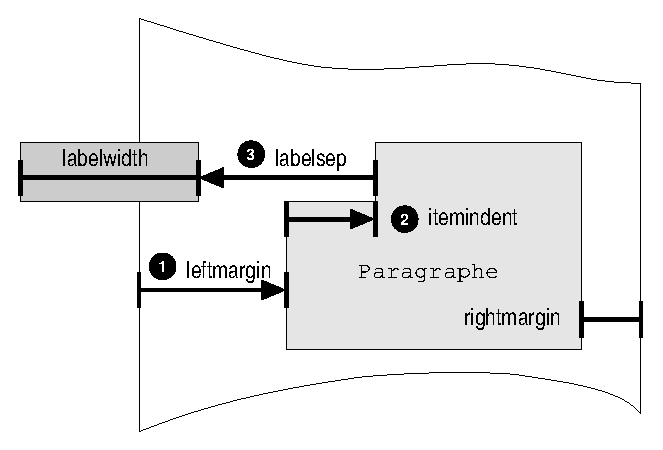
\includegraphics[width=0.4\linewidth]{img/liste-1}}
        \hspace{2cm}
        \subfloat[宽度大于\dm{\backslash labelwidth}]{%
          \label{fig:9.1b}
          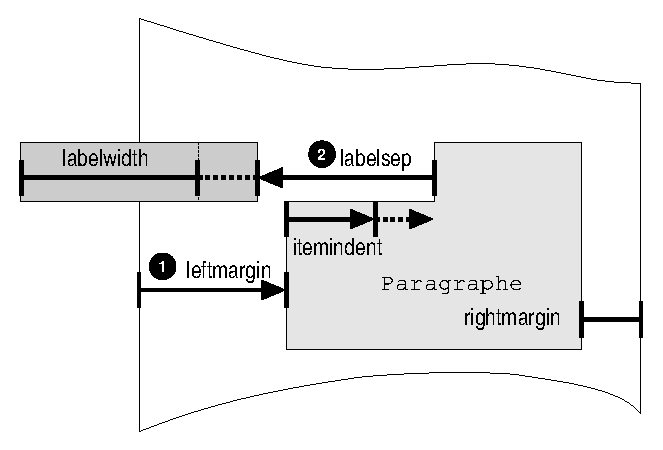
\includegraphics[width=0.4\linewidth]{img/liste-2}}
      \caption{列表入口的放置}
      \label{fig:9.1}
    \end{center}
\end{figure}

